\chapter{La señal de fonocardiograma}\label{capit:cap2}
\vspace{-2.0325ex}%
\noindent
\rule{\textwidth}{0.5pt}
\vspace{-5.5ex}% 
\newcommand{\pushline}{\Indp}% Indent puede ir o no :p



En este capítulo se conocerán las características fisiológicas del audio cardiaco, comprendiendo lo que representan cada uno de los sonidos generados así como su clasificación. De igual manera se expondrá una descripción del fonocardiograma como señal eléctrica y algunos parámetros importantes de la misma que servirán en su procesamiento digital, como la respuesta en frecuencia y forma de onda temporal. Se definirán también en esta sección las características de los sonidos que representen algún mal o anomalía en el funcionamiento del corazón, qué parámetros las caracterizan así como algunas consideraciones en su tratamiento como señal eléctrica y acústica. 

El codificador de fonocardiograma (al cual denotaremos como PCG por sus siglas en inglés) involucra diversos procedimientos en su realización. Es importante por lo tanto, conocer las características y parámetros de algunos códecs existentes; debido a esto se ha incluido en este capítulo una breve introducción a la codificación de audio en general.

De igual manera se mostrará en esta sección un breve panorama o \emph{estado del arte} en codificación de sonidos cardiacos, basado en los trabajos realizados en la literatura para el modelado y procesamiento de fonocardiogramas. Se tomarán algunas consideraciones importantes sobre estos trabajos y se definirá cuáles se han empleado en esta tesis para el desarrollo del códec.

\section{Origen fisiológico y representación de los sonidos cardiacos}

Como se ha definido anteriormente un fonocardiograma representa al audio cardiaco; se trata de una señal mecánica sonora tomada con un dispositivo médico llamado estetoscopio. Los sonidos generados por esta señal describen el comportamiento o acción mecánica de las válvulas o valvas del corazón, las cuales son compuertas que abren o cierran sistemáticamente para dar paso a la regulación de la sangre a través de las venas y arterias \cite[]{Abbas2009}. 

Existen cuatro válvulas, cada una asociada a las principales venas que están conectadas al órgano cardiaco: válvula aórtica, válvula pulmonar, válvula mitral y válvula tricúspide. Estos componentes se muestran en la Figura \ref{valvulas}.

%================================
\begin{figure}[ht]
\begin{center}
\includegraphics[width=3.3in]
{valvulas_cardiacas.jpg}
\end{center}
\par
\caption{Localización de las válvulas cardiacas. 
Tomado de \protect\url{http://www.nlm.nih.gov/medlineplus/spanish/ency/esp_imagepages/9380.htm}}
\label{valvulas}
\end{figure}
%=======================================

Son dos eventos importantes los que constituyen un PCG ordinario, denominados como S1 y S2. En el caso del primer evento o S1 se tiene un sonido que describe la actividad dada por la apertura de las válvulas aórtica y pulmonar y el cierre de las válvulas mitral y tricúspide (esto evita que la sangre circule hacia esta sección). En este evento se completa una \textbf{sístole ventricular}, donde las ventrículos se contraen para expulsar la sangre hacia las arterias \cite[]{Djebbari2000}.

El segundo evento cardiaco S2 describe el complemento de los acontecimientos dados en S1, esto es, las válvulas mitral y tricúspide ahora se abren para recibir la sangre mientras que los conductos aórtico y pulmonar se han cerrado. Este proceso se denomina \textbf{sístole aurícular} y en efecto, ahora son las aurículas quienes se han contraído para expulsar la sangre hacia los ventrículos. Se denomina \emph{ciclo cardiaco} cuando secuencialmente han ocurrido los sonidos S1 y S2. La \textbf{diástole} ocurre después de completarse un ciclo cardiaco y se trata de un periodo donde se relajan las aurículas y ventrículos. Estos dos sonidos son identificados en un fonocardiograma regular durante la actividad de un ciclo \cite[]{Abbas2009}. 
 
Existen otros dos sonidos cardiacos: S3 y S4, los cuales son asociados a otros eventos y generalmente son despreciados en el análisis del PCG. En el caso del llenado o asimilación de sangre hacia los ventrículos se origina S3, mientras que S4 ocurre al final de la diástole surgido por la contracción de las aurículas cuando han desplazado el flujo de los ventrículos \cite[]{koymen87}. 

Al espacio donde no ocurre algún evento cardiaco se le denomina \emph{silencio}.  

\section{Características del fonocardiograma}
Como señal eléctrica un fonocardiograma consta de formas de onda específicas asociadas a los sonidos cardíacos que se mencionaron anteriormente (S1 y S2). Los eventos cardíacos preservan cierta duración en tiempo y por lo tanto también contienen cierto intervalo de frecuencias, características que se muestran en la Tabla \ref{sonidosCardiacosNormales}. En la Figura \ref{ciclo} puede observarse la forma de onda de los ruidos o eventos cardiacos normales que constituyen un ciclo cardiaco. 
\begin{table}[h] 
\par
\begin{center}
\begin{tabular}{|c|c|c|}
   \hline 
   Ruido & Duración (s) & Contenido frecuencial (Hz) \\ \hline
   S1      &  0.1-0.12     & 20-150			\\ \hline
   S2      &  0.08-0.12   & 50-60			          \\ \hline
   S3      &  0.04-0.05     & 20-50			\\ \hline
   S4      &  0.04-0.05     & $<$25			\\ \hline
   \hline
   \end{tabular}
   \end{center}
   \caption{Duración y contenido frecuencial de los principales ruidos cardiacos. Tomado de \cite{castorena2012}}
   \label{sonidosCardiacosNormales}   
\end{table}

%================================
\begin{figure}[ht]
\begin{center}
\includegraphics[width=4.3in]
{ciclo_cardiaco.eps}
\end{center}
\par
\caption{Forma de onda de un ciclo cardiaco.}
\label{ciclo}
\end{figure}
%=======================================

Los sonidos cardiacos presentan cambios rápidos con respecto al tiempo y a la frecuencia debido al comportamiento no estacionario de la señal PCG. Es por esto que el estudio y entendimiento de sus características se realiza en un plano conjunto tiempo-frecuencia. La STFT\footnote{Transformada de Fourier de Tiempo Corto \emph{(Short Time Fourier Transform)}.} es una herramienta propicia para el análisis en los cambios del comportamiento del fonocardiograma \cite[]{Djebbari2000}. 

En la Figura \ref{spec_pcg} se muestra el espectrograma (gráfica de la STFT) de un ciclo cardiaco, con el cual se observa la evolución tiempo-frecuencia de los eventos S1 y S2 además de su contenido frecuencial ya antes definido. 
%================================
\begin{figure}[ht]
\begin{center}
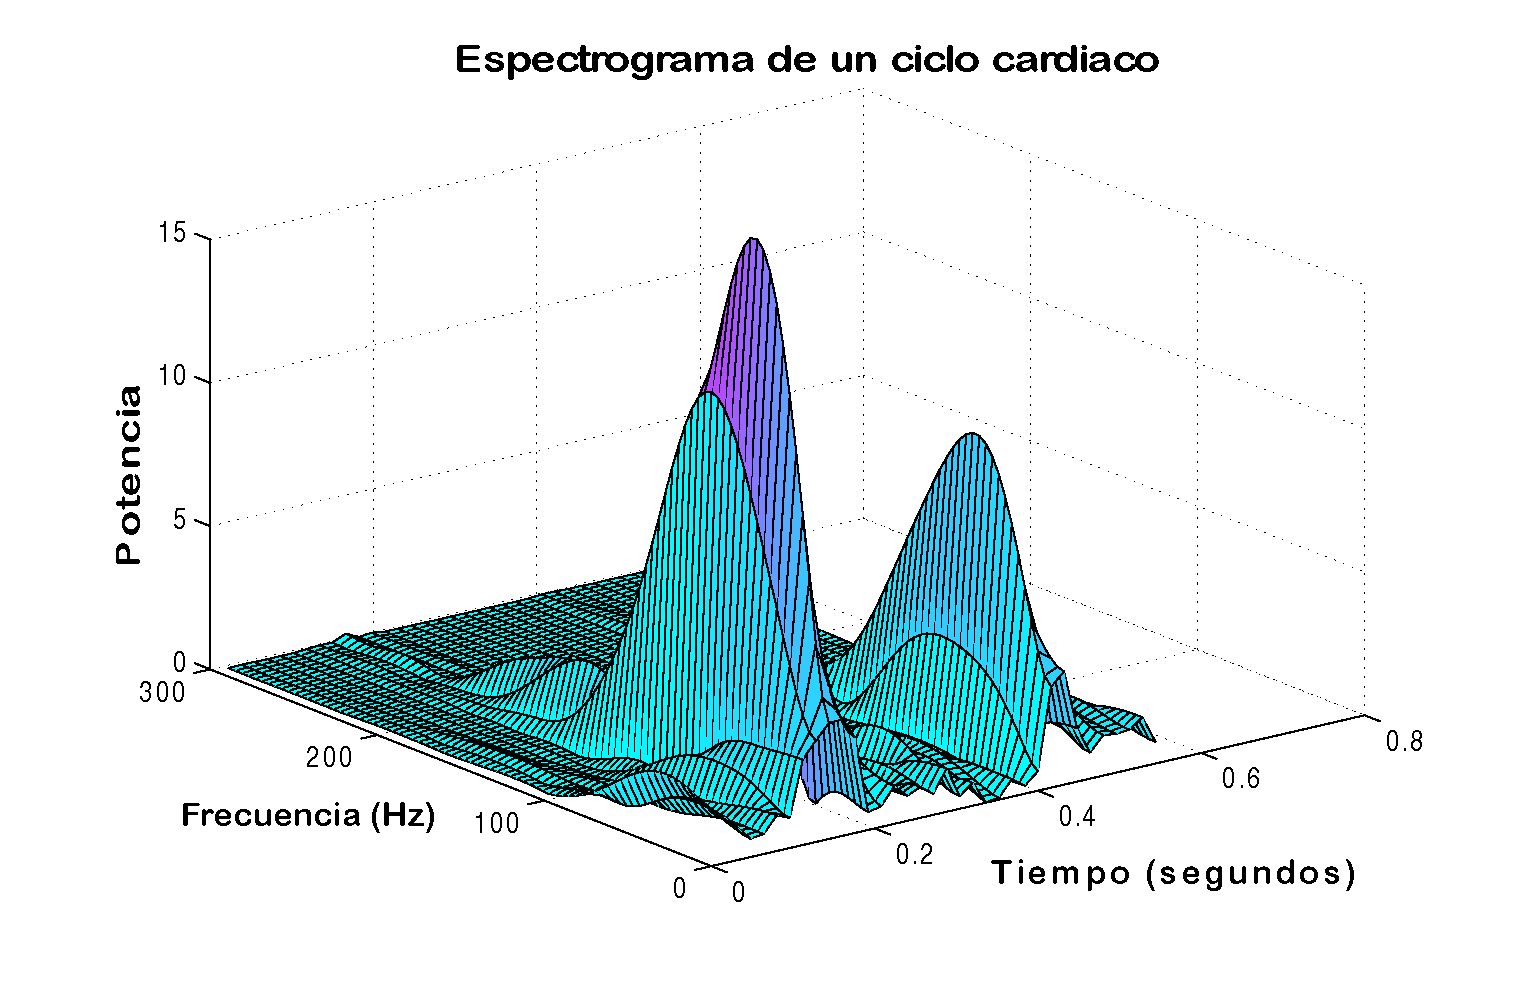
\includegraphics[scale = 0.48]{spectrogram_PCG.eps}
\end{center}
\par
\caption{Espectrograma de un ciclo cardiaco.}
\label{spec_pcg}
\end{figure}
%=======================================

La representación temporal de la envolvente de los sonidos cardiacos así como su contenido frecuencial permite identificar correctamente si se trata de eventos normales, como los que hemos mencionado en esta sección. Estos sonidos también garantizarán un funcionamiento mecánico adecuado del corazón, esto es, válvulas cardíacas trabajando adecuadamente. 

\section{Patologías cardiacas}
Las válvulas o valvas cardiacas son compuertas encargadas de regular el flujo sanguíneo a través de las aurículas y ventrículos del corazón, es por ello que la principal fuente de sonidos cardiacos anormales o patologías detectadas son daños en alguna(s) de éstas. Se distinguen principalmente dos tipos de daños valvulares en cuanto a su funcionamiento \cite{Leatham1987}. 

Particularmente son las válvulas cardiacas izquierdas las que pueden fallar al no abrir apropiadamente, a esta anomalía se le conoce como \emph{estenosis}. Por otra parte, cuando las valvas no puedan cerrar de manera adecuada se les denominará \emph{incompetentes}, provocando un bajo flujo sanguíneo o \emph{regurgitación} \cite[]{Abbas2009}. 

Los daños valvulares mencionados anteriormente producen un flujo turbulento del torrente sanguíneo a través del corazón, el cual presenta un comportamiento más brusco y puede ser percibido de manera auditiva \cite[]{koymen87}. En efecto, esto se traduce a que el PCG de una patología o anomalía cardiaca presenta cambios a frecuencias más elevadas y tiempos más cortos, teniendo alteraciones en la forma de onda y desde luego en el espectrograma. La Figura \ref{soplo_diastolico} muestra la forma de onda de una señal patológica producto de un soplo diastólico, evento que se observa entre S1 y S2 presentando a diferencia de éstos una frecuencia no tan consistente y una duración temporal mayor.
%================================
\begin{figure}[ht]
\begin{center}
\includegraphics[scale = 0.45]
{diastolic_rumble.eps}
\end{center}
\par
\caption{Forma de onda de un soplo diastólico.}
\label{soplo_diastolico}
\end{figure}
%=======================================
\section{Codificación de audio}
El sonido es un fenómeno dado por la propagación de ondas mecánicas a través de un medio, que generalmente es el aire en nuestro caso. Cualquier sonido tiene características analógicas por naturaleza, esto dado que por medio de nuestro sistema auditivo tenemos la capacidad en efecto de escuchar un sonido de manera continua \cite[]{Painter2000,Bosi2003}. 

Sin embargo, el empleo y demanda de sistemas digitales en la actualidad crea la necesidad de reproducir, transmitir, procesar y grabar al sonido digitalmente. Un \emph{códec} (codificador-decodificador) es un dispositivo que toma las señales analógicas de audio como entrada y las transforma temporalmente en una representación digital\footnote{Es decir, una cantidad adecuada (limitada) de bits para poder almacenar y representar una señal de audio.} conveniente para realizar las tareas antes mencionadas \cite[]{Bosi2003}. 

En el caso de este trabajo de tesis se requiere transmitir y almacenar señales de audio cardiaco, las cuales son producto de un fenómeno continuo y por lo tanto analógicas por naturaleza. El canal de almacenamiento y/o transmisión es limitado, la baja tasa de datos disponible hace necesaria una compresión y codificación eficiente de la señal del fonocardiograma. 

La Figura \ref{diag_codec} muestra la funcionalidad que tendrá el códec adaptado a audio cardiaco que se presenta en este documento.

%================================
\begin{figure}[ht]
\begin{center}
\includegraphics[scale = 0.46]
{diag_codec1.png}
\end{center}
\par
\caption{Esquema general del codificador-decodificador diseñado para audio cardiaco.}
\label{diag_codec}
\end{figure}
%=======================================


La codificación de audio es un proceso que requiere la digitalización de una forma de onda completamente analógica, para ello la señal deberá de sufrir diferentes procesos \cite[]{Jayant1974}. 

En la Figura \ref{dig_signal} se muestra una ilustración cualitativa de cómo una forma de onda análoga, la cual es \emph{continua} en tiempo y en amplitud es transformada al dominio digital. 

El proceso comienza con la discretización en tiempo, lo cual es conocido como \emph{muestreo}. Posteriormente se realiza la discretización en amplitud, a lo cual se le denomina \emph{cuantificación}. 

La forma de onda mostrada en la Figura \ref{dig_signal}  de la parte a) es análoga, y hasta completar el proceso en la parte d) puede apreciarse la versión digitalizada de la misma. Cada una de las muestras de la forma de onda en tiempo mostradas en d) tiene un número finito de valores de amplitud y tiempo permisibles.

La transformación de a) hacia d) puede ser por medio del paso c) y posteriormente el d) generalmente, es decir, primero se muestrea a la señal y posteriormente se cuantifica. Es importante verificar la resolución en la realización de los procedimientos anteriores, pues en efecto la señal perderá calidad y en especial durante la cuantificación, que en efecto es un proceso de compresión con pérdidas. Durante el muestreo es importante respetar el parámetro de \emph{frecuencia de muestreo} para una adecuada representación de la señal.

%================================
\begin{figure}[ht]
\begin{center}
\includegraphics[width= 6.5in]
{dig_signal.eps}
\end{center}
\par
\caption{Cuatro tipos de señales: a) Continua en amplitud y tiempo (analógica); b) discreta en amplitud y continua en tiempo; c) continua en amplitud y discreta en tiempo; d) discreta en tiempo y amplitud.}
\label{dig_signal}
\end{figure}
%=======================================


\subsection{La psicoacústica en el modelado y codificación de audio}

El diseño de los algoritmos de codificación está basado en las características del receptor, con lo cual se garantizará una optimización en la eficiencia y calidad del código. En el caso del audio el receptor es el oído humano, cuya percepción se ve afectada por sus propiedades de \emph{enmascaramiento sonoro} \footnote{Fenómeno que ocurre cuando dos o más sonidos son reproducidos simultáneamente. El más débil de ellos resultará inaudible.}. Por medio de la \emph{psicoacústica} se realiza la caracterización adecuada del sistema de percepción auditiva humana y particularmente el análisis de las capacidades tiempo-frecuencia del oído interno \cite[]{Painter2000}.

Aplicar principios de percepción del oído para la codificación de audio es realmente relevante para diversos codificadores, algunos explotan el hecho de descartar información que no es detectable para cualquier oyente bien entrenado y así comprimir la señal \cite[]{Schroeder1979}. Esta información irrelevante se identifica durante el análisis de señal incorporando en el codificador principios psicoacústicos como umbrales absolutos de audición, análisis de bandas de frecuencia críticas, enmascaramiento simultáneo y temporal, entre otros. 

El umbral absoluto de audición caracteriza la cantidad de energía necesaria en un tono puro tal que pueda ser detectado por un oyente en un ambiente sin ruido. La \mbox{Figura \ref{umbral_audicion}} muestra el comportamiento del umbral de audición absoluto en el espectro frecuencial. Dicha gráfica es el resultado de cuantificar el nivel de presión de sonido (SPL) requerido para cada frecuencia detectada por el oyente (tono puro).
%================================
\begin{figure}[ht]
\begin{center}
\includegraphics[scale = 0.86]
{umbral_audicion.pdf}
\end{center}
\par
\caption{Umbral absoluto de audición. Tomado de \cite{Painter2000}.}
\label{umbral_audicion}
\end{figure}
%=======================================

\subsection{El códec de audio}
Como mencionamos anteriormente un códec de audio es el sistema que incluye el conjunto de algoritmos para permitir codificar y decodificar datos auditivos en una cantidad limitada de bits \cite[]{Bosi2003,Painter2000}. Es importante que un códec pueda comprimir el archivo de audio para ocupar el menor espacio posible y una calidad aceptable para reproducirlo adecuadamente \cite[]{Painter2000}. Los siguientes parámetros son importantes en la definición de un códec de audio:
\begin{itemize}
	\item\textbf{Número de canales.} Esto se refiere al número de señales simultáneas de audio que contiene el flujo de datos. De acuerdo a ello la señal puede ser mono (un canal), estéreo (dos canales) o multicanal 5.1 (6 canales) ó 7.1 (8 canales).
	\item\textbf{Frecuencia de muestreo.} Una señal analógica de audio necesita ser discretizada primeramente en el tiempo, para ello se emplea el muestreo. El teorema de Nyquist establece que la frecuencia de muestreo adecuada para representar una señal debe ser el doble de la frecuencia máxima contenida en el ancho de banda de la señal. Ejemplos de ello son los estándares MPEG-3 (MP3), el cual muestrea con calidad de CD a diferentes frecuencias de muestreo; la más común es de 44,100 Hz teniendo en cuenta que el oído humano no es capaz de escuchar frecuencias superiores a 22 kHz.
	\item\textbf{Número de bits por muestra.} Con ello se determina qué precisión existe al reproducir la señal original así como el rango dinámico de la misma. Suelen utilizarse en los codificadores convencionales 8, 16 ó 24 bits por muestra aunque en calidad CD comúnmente se emplean 16. 
	\item\textbf{Tipo de compresión.} Se distingue entre compresión con pérdidas (\emph{lossy compression}) y sin pérdidas (\emph{lossless compression}).
		\begin{itemize}
		\item \emph{Compresión con pérdidas}: La información que se considera irrelevante es despreciada, aunque con ello es evidente 					tener una pérdida en la calidad del resultado al ejecutar la decodificación final.		
		\item \emph{Compresión sin pérdidas}: Toda la información es transmitida, sólo se elimina la información repetida o redundante y la 								información que no se repite se almacena ocupando un menor espacio.
		\end{itemize}
		
	\item\textbf{Tasa de bits (datos).} Esta cantidad determina el número de bits necesarios por unidad de tiempo y no puede deducirse a través de los parámetros anteriores, ya que pudo aplicarse una compresión con o sin pérdidas. De acuerdo a su estabilidad puede ser \emph{constante (CBR)} o \emph{variable (VBR)}. VBR es de uso más frecuente en audio y además más eficiente que CBR ya que existen tramos de silencios aleatorios donde deberá bajar la cantidad de bits a transmitir y por lo tanto variar la tasa. 
		\begin{itemize}
		\item\emph{Tasa de bits constante (CBR)}: La tasa de salida del codificador es constante. CBR es útil en en flujo de datos multimedia para canales de capacidad limitada, sin embargo no es la mejor opción para almacenamiento, ya que no asigna suficientes bits para las secciones complejas (por lo tanto se degrada la calidad) además de usar bits innecesarios en secciones de menor complejidad.
		\item\emph{Tasa de bits variable (VBR)}: En este método de compresión se consigue una mayor calidad de sonido para un tamaño de archivo determinado. En contraste a CBR se otorga la tasa de bits necesaria a cada parte del archivo que se pretende codificar consiguiendo una calidad mayor en archivos de tamaño reducido. Al codificar con VBR, el codificador asignará las tasas de bits que variarán según la complejidad de la onda de audio a lo largo del archivo. Este formato es muy apropiado para la transmisión de audio en tiempo real.
		\end{itemize}
\end{itemize}
En la actualidad existen diversos códecs de audio, aunque cada vez son más complejos y presentan características adicionales a las mencionadas anteriormente. De acuerdo a los parámetros existentes en algunos codificadores de audio expuestos por \cite{Bosi2003}, se ha realizado en esta tesis una clasificación en cuatro grandes grupos:
\begin{itemize} 
	\item \textbf{Codificadores de forma de onda.} Estos codificadores están basados en el estudio general de la señal, de tal manera que intentan reproducir la forma de la señal de entrada \cite[]{OReilly1984}. Son diseñados en general para ser independientes de la señal, de manera que puedan ser útiles para  codificar una variedad extensa de señales; la redundancia de la señal es aprovechada para lograr una compresión. 
		
	Algunos codificadores de forma de onda son:			
	\begin{itemize}
				\item Modulación por codificación de pulsos (\emph{Pulse Code Modulation} ó PCM). Esta codificación es la base para la 						mayoría de los codificadores y a la vez se incluye en el procedimiento para digitalizar una señal. Basta con 							representar mediante impulsos las variaciones en amplitud de las muestras de la señal de entrada.
				\item Modulación diferencial por pulsos codificados (DPCM). Basándose en el principio de PCM, DPCM codifica solamente la 						diferencia entre la muestra presente y la muestra anterior de la señal de entrada. Se envía una cantidad mayor de 						información y un número más reducido de bits si se compara con PCM, sin embargo si existe un error en alguna 						trama codificada con PCM éste afectará tanto a la muestra actual y las muestras subsecuentes.
				\item Modulación diferencial adaptativa por pulsos codificados (ADPCM). Se trata de una variante de DPCM donde se varía la 					escala de codificación según las diferencias entre las muestras actual y subsecuente, es decir se asignan cantidades 						variables de bits a éstas según corresponda.
			\end{itemize}
Algunos codificadores de forma de onda basados en PCM u otras de sus variantes han tenido éxito para transmitir señales de voz sobre canales telefónicos. Ejemplos de éstos son el codificador $\mu-255 PCM$ \cite[]{Dammann1972} y el $G722$ \mbox{\cite[]{Mermelstein1988}}.  

	\item \textbf{Codificadores perceptuales.} Se aprovechan las limitaciones en la percepción del sistema auditivo humano para codificar el flujo de datos. Las muestras son codificadas en formato PCM y son convertidas al dominio de la frecuencia. Dada esta conversión la señal puede descomponerse en sub-bandas y proporcionar una resolución mayor a las bandas de frecuencia donde el oído humano sea más sensible. 
	La codificación puede también llevarse a cabo por transformada, codificando las componentes de una transformada unitaria de la señal realizando la operación inversa (antitransformada o transformada inversa) en el decodificador. En este caso la compresión se presenta debido a lo no correlacionadas que tienden a ser las componentes generadas por las transformadas unitarias de manera que pueden codificarse independientemente.
Otra manera útil de desechar información irrelevante al codificar audio de manera perceptual es la codificación en \emph{sub-bandas}, pasando la señal de audio por diversos filtros pasa-banda a diferentes frecuencias para codificarla de manera independiente y dar diferente resolución a las bandas más sensibles.

Se muestra en la Figura \ref{cod_perceptual} el diagrama a bloques que ilustra el procedimiento de codificación de audio de manera perceptual.
%================================
\begin{figure}[ht]
\begin{center}
\includegraphics[scale = 0.66]
{diagCodPerceptual.pdf}
\end{center}
\par
\caption{Diagrama a bloques de un codificador de audio perceptual.}
\label{cod_perceptual}
\end{figure}
%=======================================

El grupo de trabajo \textbf{Moving Picture Experts Group (MPEG)} ha establecido diversos estándares para la transmisión de audio, aprovechando en ellos la codificación perceptual para diseñar codificadores como MP3 \cite[]{Musmann2006,Noll1997}. Otro codificador perceptual de audio que ha tenido reconocimiento en el mercado es el \emph{Advanced Audio Coding (AAC)} \cite[]{Bosi1997}.

	\item \textbf{Codificadores paramétricos.} Estos codificadores se basan en el hecho de que el audio y la voz pueden representarse y sintetizarse como tonos aislados o patrones armónicos, esto es, representarlos con ondas senoidales y componentes ruidosas (\emph{sinusoid plus noise modeling}). Los parámetros de las sinusoides son los que se codifican: amplitud, frecuencia fundamental o componentes espectrales. Estos parámetros requieren por lo general pocos bits para ser representados \cite[]{Quatieri1985,McAulay1986,RuizReyes2010}. 
	
	En la Figura \label{cod_parametrico} se muestra el diagrama a bloques de un codificador de audio tipo paramétrico.
		%================================
		\begin{figure}[ht]
		\begin{center}
		\includegraphics[scale = 0.66]
			{diagCodParametrico.pdf}
		\end{center}
		\par
		\caption{Diagrama a bloques de un codificador de audio paramétrico.}
		\label{cod_parametrico}
		\end{figure}
		%=======================================
	\item \textbf{Codificadores híbridos.}  Combinan las técnicas de los codificadores de forma de onda para obtener la 				señal de audio de más alta calidad con tasas bajas de bits. Un conjunto de muestras es analizado como si se tratase de una sola 				para obtener los parámetros de la señal. Cuando la trama se decodifica los parámetros son sintetizados para conseguir que se 				parezca al original. Se conocen algunos codificadores híbridos de la literatura:
		\begin{itemize}
			\item El vocoder (codificador de voz) basado en la técnica \emph{Residual-Excited Linear Prediction (RELP)} desarrollado por 						\cite{Un1975}.
			\item Algunos codificadores de voz basados en el algoritmo \emph{Code Excited Linear Prediction (CELP)}, donde se emplean diccionarios o bloques de código adaptativos \cite[]{Mano1995,Kipper1991,Miki1994,Koishida1996}.
			\item Codificadores que emplean predicción lineal mediante suma de vectores, conocidos como\emph{Vector Sum Excited Linear Prediction (VSELP)}. Algunos de ellos han sido desarrollados por \cite{Gu1995,Sunwoo1991,Choi1996,Gerson1990}.
			\item Codificación mediante el método \emph{Regular Pulse Excitation-Long Term Prediction (RPE-LTP)}. Los codificadores diseñados por \cite{Huerta2001a,McLoughlin2000,Coleman1989} se basan en esta técnica. 
		\end{itemize}	
\end{itemize}

En este trabajo de tesis se desarrollará un codificador tipo \emph{paramétrico} con pérdidas aprovechando la alta correlación existente entre los eventos del audio cardiaco y las formas de onda conocidas como átomos de Gabor. La siguiente sección describe las técnicas que se han usado en la literatura para el modelado del fonocardiograma.

\section{Estado del arte en el modelado de sonidos cardiacos}
La primer parte para el diseño de un codificador de audio cardiaco paramétrico consiste en el modelado matemático, el cual dotará de características propias y codificables al PCG además de encontrar la representación más adecuada y que represente mayor compresión. 
Robert Hooke, conocido por sus trabajos en elasticidad de materiales, otorgó potencialidad en el diagnóstico de patologías a la auscultación cardiaca \cite[]{Wood1995}. Y es que Hooke fue capaz de escuchar claramente los sonidos pertenecientes a los latidos del corazón y planteaba que tal vez pudiese indagar sobre el funcionamiento de otros órganos del cuerpo humano mediante el sonido que éstos generaban \cite[]{Leatham1987}.

El estetoscopio fue creado por Laënnec en 1816 \cite[]{Roguin2006} e hizo del fonocardiograma una herramienta fundamental en la diagnosis clínica hasta nuestros días. Sin embargo, la escasez de estándares en la nomenclatura, los transductores empleados en el registro y las locaciones para llevarlo a cabo mostraron un progreso lento; como resultado se tuvo un pobre entendimiento de los mecanismos del sonido cardiaco y la inherente complejidad de los sonidos cardiacos. 

Sin embargo, algunos factores han hecho del PCG una herramienta de diagnóstico limitada. La percepción auditiva humana es la primer limitante; aunque los especialistas y cardiólogos muestren singulares habilidades en el reconocimiento de diversas patologías no se garantiza que la auscultación tenga una precisión para diagnosticar. En efecto, toda señal de audio es pasa-bajas, de baja intensidad para el oído humano y muy corta duración. La banda baja de frecuencias puede concentrar también información importante del fonocardiograma.
 
 Los avances en el procesamiento digital de señales así como la aparición del diagnóstico asistido por computadora (\emph{Computer-Aided Diagnosis}) han logrado reforzar al PCG para ser una herramienta importante en el estudio de anomalías cardiacas. Los estetoscopios actuales muestran ahora las formas de onda y el análisis de la señal es más extenso \cite[]{Mahnke2009,Watrous2008}.
 
 Algunos trabajos en la literatura han realizado un análisis extenso en el plano tiempo-frecuencia del PCG, mostrando una caracterización espectral del mismo ya sea por espectrogramas calculados por la STFT o distribuciones Wigner-Ville \cite[]{Ghofrani1993}, tal es el caso de \cite{Djebbari2000,Debbal2007,Debbal2008} y \cite{Jasper2010}. En otros trabajos como los realizados por \cite{Boutana2011} y \cite{DEBBAL2006} se realiza la identificación de cardiopatologías usando como herramientas las distribuciones tiempo-frecuencia antes mencionadas.
 
 De acuerdo a lo mencionado en las secciones anteriores de este trabajo con respecto al PCG se trata de una señal no estacionaria, esto es, los ciclos cardiacos no son consistentes en posición, duración temporal ni contenido frecuencial. Dada esta característica los autores se han dedicado a analizar las componentes principales por separado: los primeros eventos cardiacos (S1) son estudiados en los trabajos de \cite{Chen1997,Wood1995} y \cite{Wood1992}, mientras que los trabajos de \cite{Hedayioglu2012,wang04} han estudiado de manera específica el comportamiento del evento S2.
 
 Se ha propuesto en el trabajo de \cite{koymen87} un modelado del PCG a partir de sinusoides amortiguadas, dadas que las estructuras en el pecho (lugar donde se realiza la auscultación) y venas de mayor contribución constituyen un sistema selectivo en frecuencia excitado por la aceleración y desaceleración de las válvulas. 
 
 El modelado del fonocardiograma mediante senoidales amortiguadas se ha extendido en la literatura para realizar diversos procesos en el PCG tales como eliminación de ruido (\emph{denoising}), segmentación de eventos, separación de componentes (diagnóstico de cardiopatologías así como la división de los eventos S1 y S2) y escalamiento en el plano tiempo-frecuencia \cite[]{Nieblas2013,Zhang1998b,Zhang1998a,Sava1998}.
 
  Los trabajos anteriormente citados emplean el algoritmo \mbox{\textbf{Matching Pursuit}} \cite[]{Mallat1993} con éxito en el análisis y síntesis del fonocardiograma, tal método selecciona un conjunto de formas de onda cosenoidales (cuyo \emph{amortiguamiento} viene dado por la modulación mediante una ventana gaussiana) denominadas \emph{átomos de Gabor} pertenecientes a un bloque conocido como diccionario. 
   
 La compresión de fonocardiogramas es el paso donde se extraen los parámetros más importantes del modelado de señal para representarlos de manera digital. Otros autores de la literatura han realizado este procedimiento efectuando la representación del audio cardiaco mendiante ondeletas (en Inglés \emph{wavelets}) como \cite{Alajarin2004,Alajarin2005,Martinez-Alajarin2006}, además de realizar también por el mismo método el proceso de \emph{de-noising} \cite[]{Messer2001}. 
 
 Por otra parte, en la tesis desarrollada por \cite{castorena2012} se propone adaptar códecs ya existentes para trasmitir el audio cardiaco sobre diversos escenarios que involucran redes con bajas tasas de datos. Posteriormente \cite{Nieblas2014} analizó diversos bloques de ondeletas mediante Matching Pursuit para elegir el que represente a la señal PCG de la manera más adecuada. 
 
 No obstante, hasta el momento no se conoce que se haya diseñado algún codificador de audio cardiaco, se ha revisado en esta sección que el modelado y la compresión del PCG han sido explorados quedando pendiente la realización de un códec que permita describir en bajas tasas de datos a esta señal para su transmisión en redes de bajos recursos.
 
  En el siguiente capítulo se aplicará la compresión de fonocardiogramas mediante \mbox{\textbf{Matching Pursuit}}, ya que conforma una parte medular del codificador a diseñar en esta tesis.
  

